\documentclass[11pt,a4paper,twoside]{article}
\usepackage[utf8]{inputenc}
\usepackage{amsmath}
\usepackage{amsfonts}
\usepackage{amssymb}
\usepackage{graphicx}
\graphicspath{{../figures/}}
\usepackage{booktabs}
\usepackage{parskip}
\usepackage{hyperref}
\setlength{\parskip}{1em}
\usepackage{nth}
\renewcommand*\familydefault{\sfdefault}
%\setsecnumdepth{subsection}
%\usepackage{chngcntr}
\usepackage{siunitx}
\DeclareSIUnit{\gu}{gu}
%\usepackage[left=2cm,right=2cm,top=2cm,bottom=2cm]{geometry}
\usepackage{bm}
\setcounter{section}{0}

\newcommand{\be}{$\bm{E(r,t)}$\,\,}
\newcommand{\cy}{$\mathrm{Y}$}
\newcommand{\cz}{$\mathrm{Z}$}
\newcommand{\rmd}{\mathrm{d}}
\newcommand{\rme}{\mathrm{e}}
\newcommand{\ISF}{I_{\mathrm{SF}}}
\newcommand{\wSF}{\omega_{\mathrm{SF}}}
\newcommand{\IIR}{I_{\mathrm{IR}}}
\newcommand{\wIR}{\omega_{\mathrm{IR}}}
\newcommand{\IVIS}{I_{\mathrm{Vis}}}
\newcommand{\wVIS}{\omega_{\mathrm{Vis}}}
\newcommand{\Gam}{\bm{\Gamma}^{(2)}(\wSF)}
\newcommand{\focal}{f_{\mathrm{focal}}}
\newcommand{\zR}{z_{\mathrm{R}}}
\newcommand{\dfocal}{\Delta z_{\mathrm{focal}}}
\newcommand{\IVISO}{I_{\mathrm{Vis,0}}}
\newcommand{\IIRO}{I_{\mathrm{IR,0}}}
\newcommand{\erfc}{\mathrm{erfc}}
\usepackage[side]{footmisc}
\usepackage{xfrac}
\usepackage{xcolor}
\usepackage{caption}
\usepackage{subcaption}

\usepackage{tikz}
\usetikzlibrary{shapes.geometric, arrows}

\tikzstyle{startstop} = [rectangle, rounded corners, minimum width=3cm, minimum height=1cm,text centered, draw=black, fill=red!30]
\tikzstyle{io} = [trapezium, trapezium left angle=70, trapezium right angle=110, minimum width=3cm, minimum height=1cm, text centered, draw=black, fill=blue!30]
\tikzstyle{process} = [rectangle, minimum width=3cm, minimum height=1cm, text centered, text width=3cm, draw=black, fill=orange!30]
\tikzstyle{decision} = [diamond, minimum width=3cm, minimum height=1cm, text centered, text width=4cm, draw=black, fill=green!30]
\tikzstyle{arrow} = [thick,->,>=stealth]



\begin{document}
\title{Liquid Surface Height Controller - User Manual v1.0}
\maketitle

\tableofcontents
\section{Introduction}
The Liquid Surface Height Controller (LSHC) is intended for use in sum-frequency generation (SFG) spectroscopy experiments conducted at liquid interfaces. At such interfaces, the height of the liquid constantly drops over time as the liquid evaporates. The instrument described here provides a way to automatically monitor and correct for this evaporation using a laser pointer, USB webcam, and syringe pump. The instrument is controlled using a LabVIEW program described herein.

The working principle of the system is shown in \autoref{fig:incidentangles}\,(a). A laser beam reflected from the surface of a liquid hits a CCD sensor. Any change in the height of the surface $\Delta h$ results in a corresponding change to the position of the reflected beam on the CCD $\Delta r$. The size of $\Delta r$ for a given $\Delta h$ depends on the angle of incidence, $\theta$. Straightforward trigonometry shows that:
\begin{equation}\label{eq:angle}
\Delta r = \sec \theta \Delta h
\end{equation}
Larger angles of incidence $\theta$ produce a larger $\Delta r$ for a given $\Delta h$.

\begin{figure}
\centering
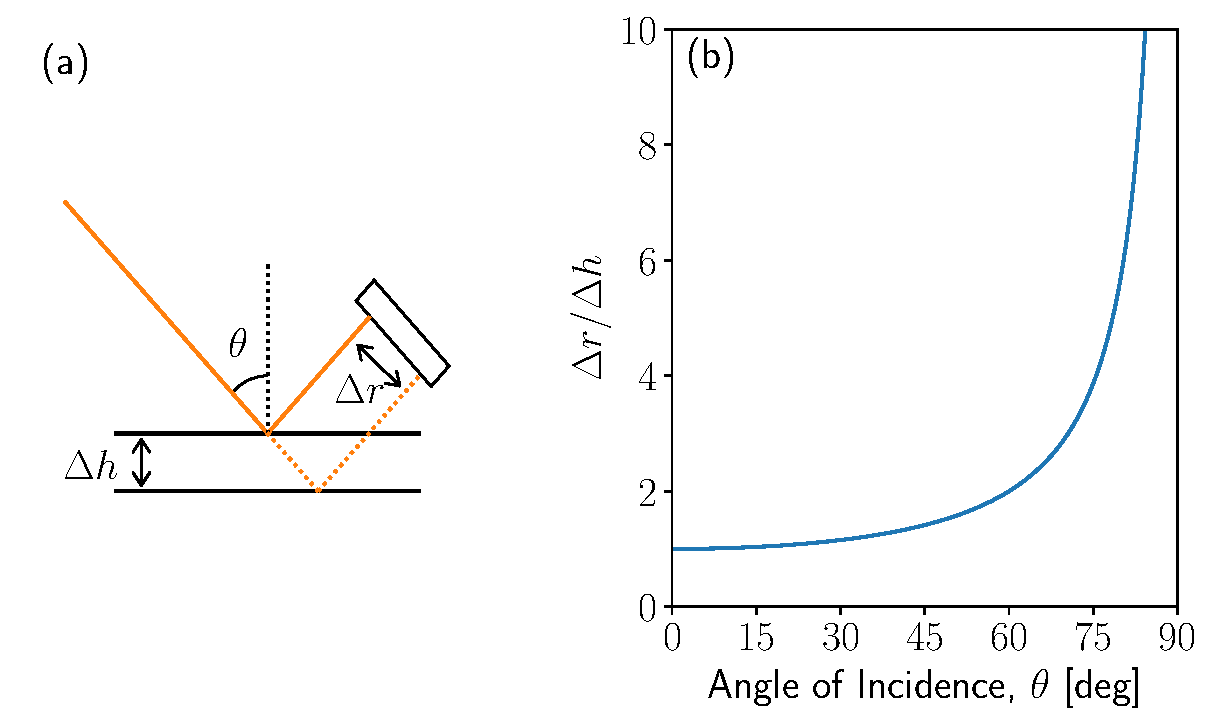
\includegraphics[width=\textwidth]{incident_angles.pdf}
\caption{(a) Sketch of the working principle of the system. (b) graph of the sensitivity $\Delta r /\Delta h$ as a function of the incident angle $\theta$.}\label{fig:incidentangles}
\end{figure}

\section{Hardware}
A 3D model of the hardware used in the setup is shown in \autoref{fig:3dmodel}. Note that different kinds of hardware could be used with the same setup, and here we describe both the hardware used in Aarhus University, and what other kinds of hardware could be used.

\begin{figure}
\centering
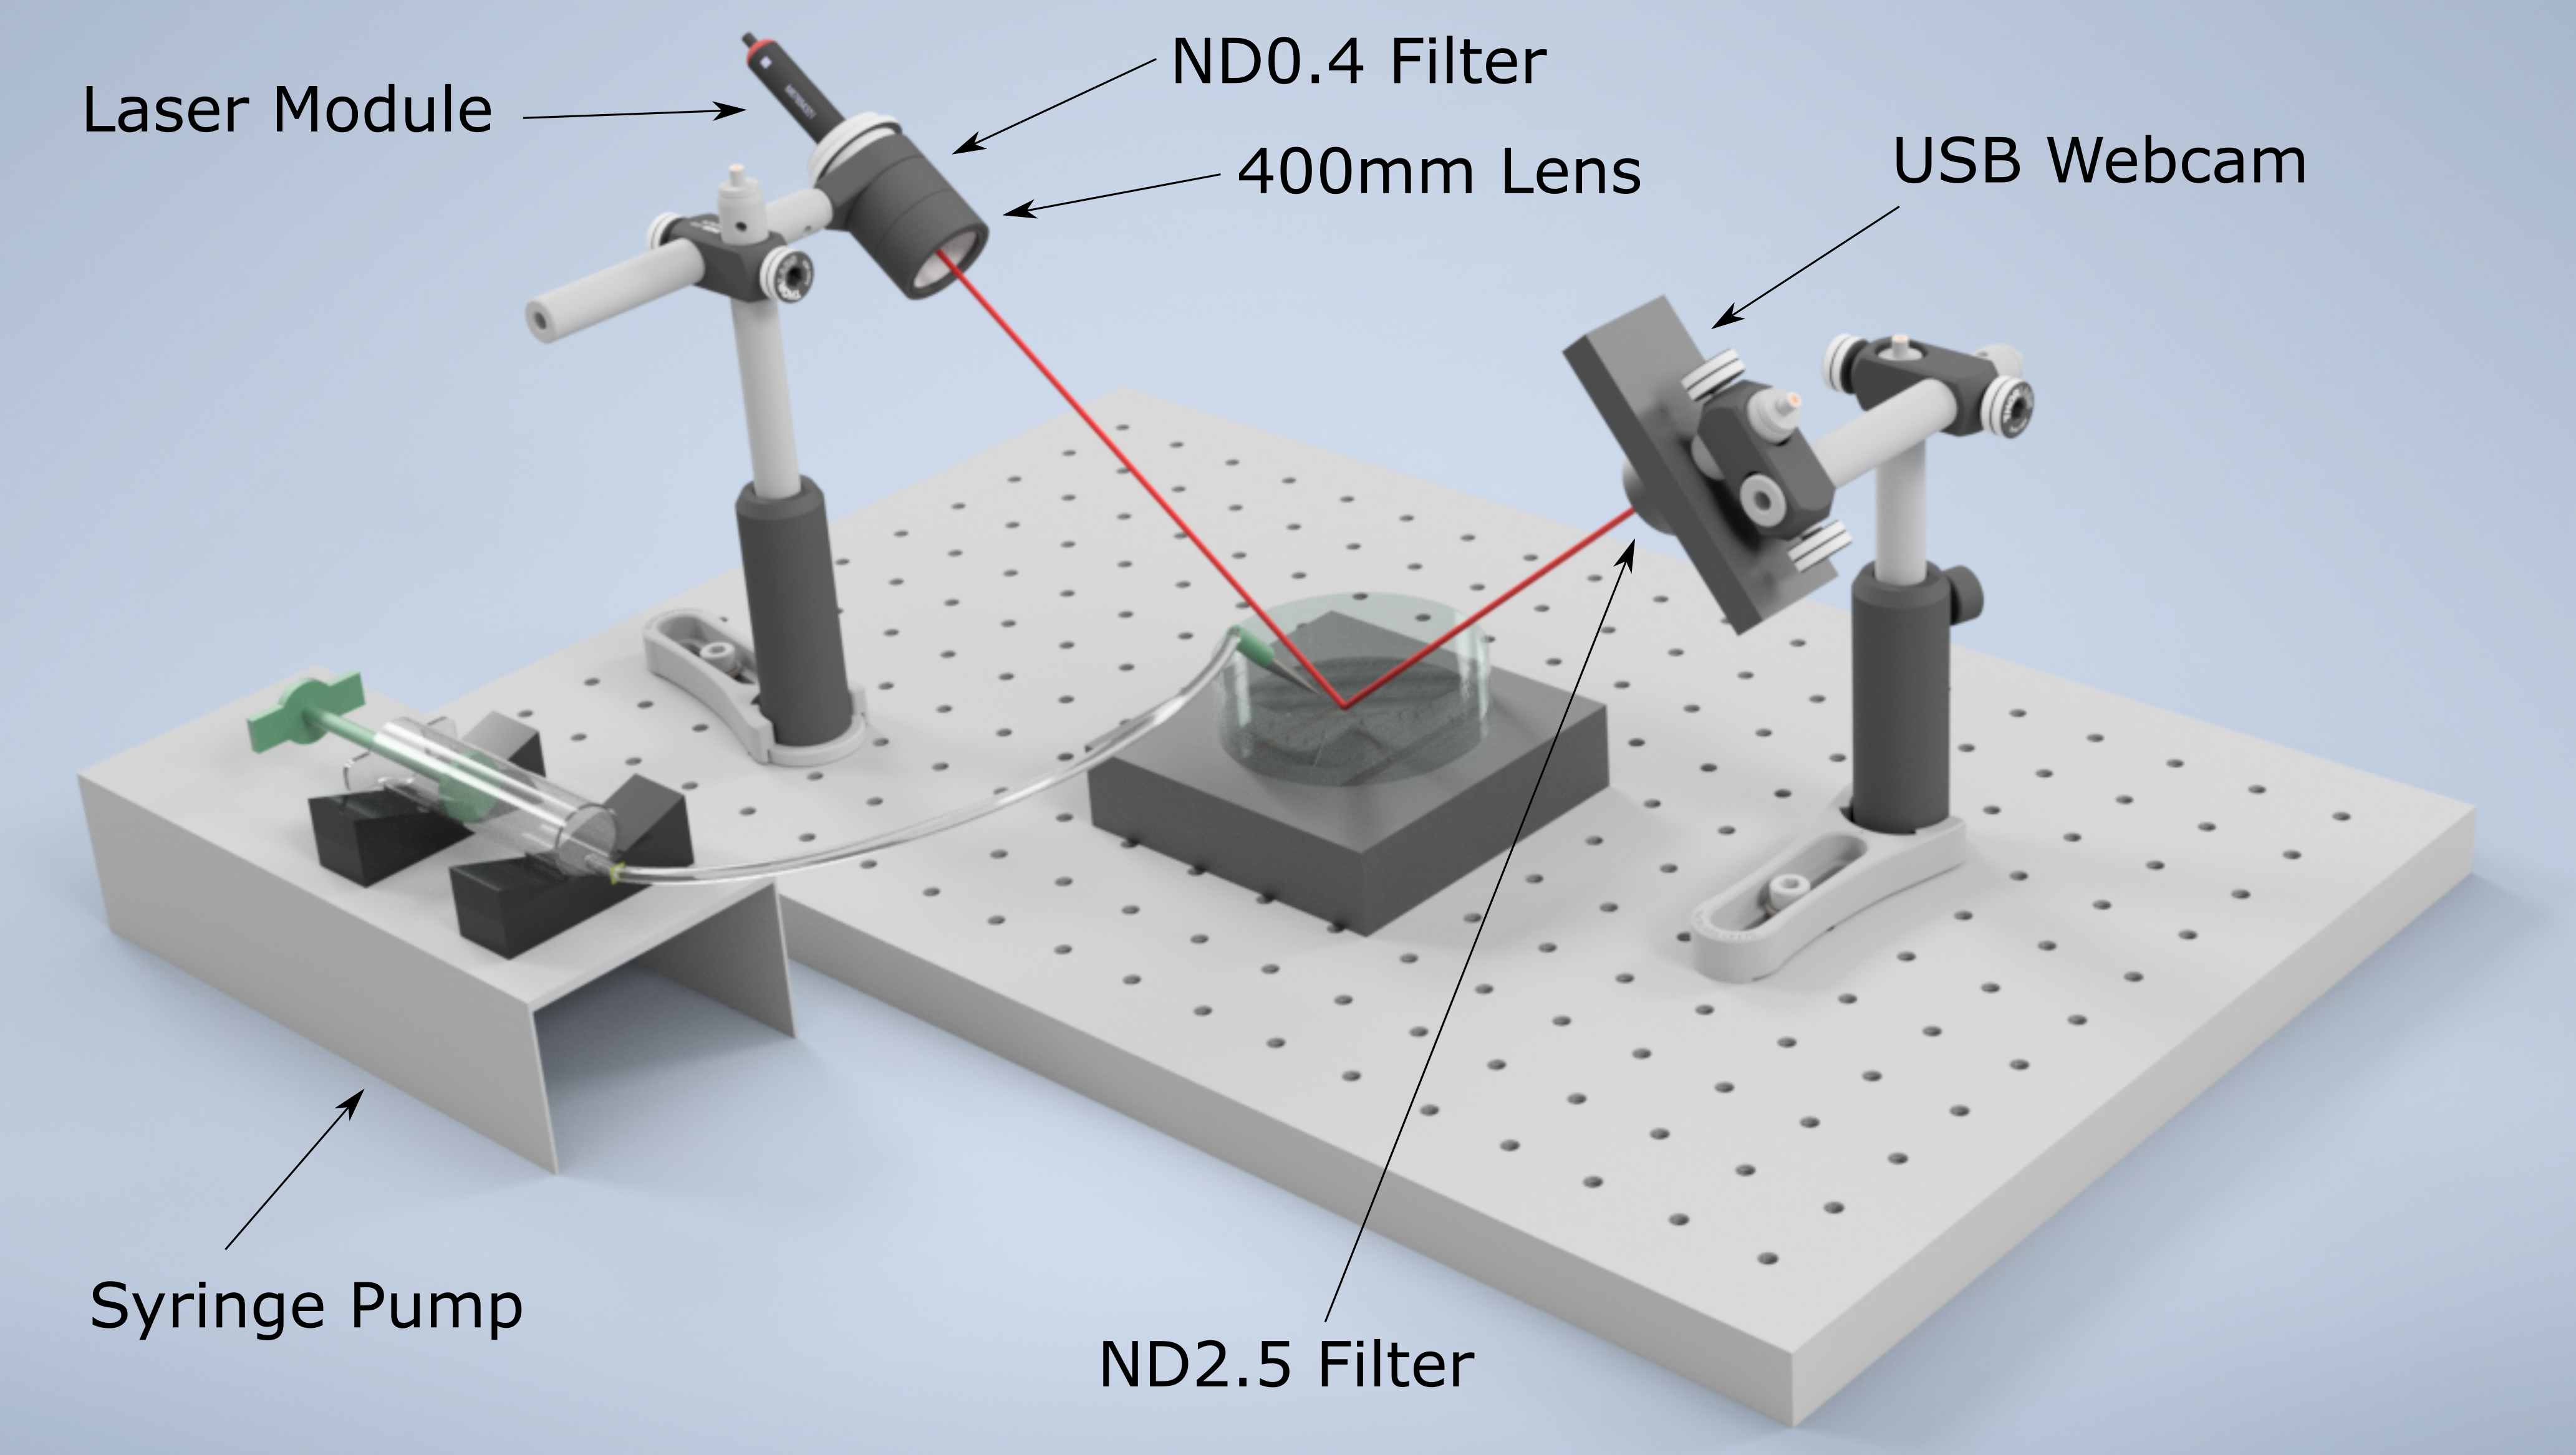
\includegraphics[width=0.8\textwidth]{heightsensor_pump_label.png}
\caption{3D model of the hardware used for the LSHC.}\label{fig:3dmodel}
\end{figure}

\subsection{Laser Source}
The laser source (on the left in \autoref{fig:3dmodel}) can, in principle, be any laser pointer that produces a sufficiently small and collimated beam. To this end we have used laser modules from the Thorlabs PL range, specifically the PL202. In choosing a laser source, the key characteristics to consider are:
\begin{itemize}
\item \textbf{Beam Quality:} the beam must be smaller than the CCD sensor, and not be so divergent that compensation for it with standard lenses is challenging. A beam with a beam waist radius of \SI{1}{\milli\metre} or less is desirable.
\item \textbf{Output Power:} the output power should be low enough that a reflection from the liquid interface does not saturate or burn the CCD, nor damage the liquid interface. In practice any low power (\SI{1}{\milli\watt} or less) will work provided that ND filters can be used in front of the laser/webcam to avoid saturation.
\item \textbf{Output Wavelength:} the output wavelength must be such that it does not interfere with the experiment, either by affecting photochemistry on the sample surface, or by overlapping with the colour of the detected light. Having several sources that fit into the same mounting, with different output wavelengths, can be advantageous in this regard.
\end{itemize}

Note that very inexpensive laser diodes often produce beams that are highly divergent along one axis and so would be inappropriate for this use without use of an anamorphic prism pair (or similar) to compensate for the ellipticity. 

There must be a way to mount a focussing optic on the front of the laser pointer, preferably with an adjustable distance from the laser output, so that any divergence or focussing/defocussing caused by the liquid surface can be compensated for. Using a mount such as the Thorlabs KAD11F makes this easy, and any 1 inch optic can be mounted onto the SM1 threading. SM1 threaded spacers can then be used to control the distance of the lens from the laser output. Other optics such as filters or irises can also be mounted on this threading if needed. The example shown in \autoref{fig:3dmodel} has an ND0.4 filter (to reduce the power) and a \SI{400}{\milli\metre} singlet lens mounted on it. 

\subsection{USB Camera}
The USB camera (on the right in \autoref{fig:3dmodel} can also, in principle, be any USB webcam that has sufficient resolution and can run sufficiently fast. We have used a Sandberg 1080p webcam, that was chosen as it was inexpensive and readily available at a local supplier. In choosing a webcam, the key characteristics to consider are:
\begin{itemize}
\item \textbf{CCD Size:} have a sufficiently large CCD that the incoming beam does not completely fill it - most webcams have CCD chips which are are around \SI{3}{\milli\metre} long along the longest axis, this is sufficient for most purposes. Larger CCDs will extend the working range of the device. 
\item \textbf{CCD Resolution:} having sufficient resolution that small changes in the height can be distinguished. Anything running at 720p or 1080p is sufficient in this regard. 
\item \textbf{CCD Speed:} readout at \SI{30}{\hertz} or more is desirable, but slower readout speeds would also work. Note that the slower the readout speed, the more measurements it will take to average out the effect of instantaneous fluctuations in the height.
\item \textbf{Connectivity:} USB connectivity is needed for the webcam to interface with the provided LabVIEW program.
\item \textbf{Adaptability:} Removal of the webcam focussing lens to expose the bare CCD is required. This is easier on some webcams than others. Being able to mount the camera on standard optomechanical mounts is almost essential.
\end{itemize}

It is critical to be able to not only remove the focussing lens, but also mount an ND filter in its place. This filter has the effect of removing ambient light (which causes a large and often non-uniform background on the measured image), and also prevents the CCD from being saturated or burned by the incident laser beam. To mount the filter the mechanical workshop in Aarhus Chemistry machined a push fit aluminium filter holder to fit where the focussing lens used to sit. You will probably be surprised at how little light is needed to produce a measurable image on the CCD. 

The camera image is read and processed via LabVIEW IMAQ subvis, and most USB webcams are compatible with these. Note that Raspberry Pi NoIR cameras, which are appealing due to their small footprint, are sometimes tricky to run in peripheral mode (as a USB device) in our experience can only run at around \SI{2}{\hertz} in LabVIEW without more user programming.


\subsection{Syringe Pump}
The constraint on the syringe pump is that in the provided LabVIEW program, drivers designed to operate pumps from \url{http://syringepump.com/} are used to control the pumping. It would be possible to modify the LabVIEW to work with other pumps (or indeed, other ways to compensate for height changes), but these have not been hard coded into the existing software. The pump used in our system is the NE-500 Programmable Syringe Pump from the company linked above.

\subsection{Sample Holder}
The system can maintain the height of a liquid surface in any sample holder with an open top (not behind a lid), within reason. There are two considerations to be aware of when using certain sample holders:
\begin{itemize}
\item Sample holders with a very small surface area can cause extreme curvature of a liquid surface due to meniscus formation.
\item Sample holders that are very shallow (and with a reflective base) will produce two reflections, from the liquid surface, and the base of the holder.
\end{itemize}
Neither of these points are catastrophic provided they are compensated for. In the first case, it may be necessary to use a relatively strong focussing/defocussing lens before the sample to account for the defocussing/focussing of the reflected beam caused by the surface curvature. It can take some trial and error to find an appropriate lens, and this should be factored into setup time. 

In the second case, the solution is simply to ensure that the beam imaged on the webcam actually comes from the liquid interface and not the sample holder. This is easily tested by changing the liquid level and seeing if the beam moves; or disturbing the liquid surface and seeing if the beam moves. If both reflected beams are visible by eye, simply taking the higher of the two, or using a razor blade/beam block to block the lower one, is also an easy solution.

\section{Software}
The software provided is written in LabVIEW 2020. The overall workflow of the program is:
\begin{equation*}
\text{Read CCD Image} \rightarrow \text{Find Centre} \rightarrow \text{Compare to Reference} \rightarrow \text{Compensate for Drift}
\end{equation*}
The LabVIEW program is provided at the following LINK. The control logic and workings of the program are now explained in more detail. 
\subsection{Control Logic}
Initially, the image on the CCD is read by LabVIEW, and the luminance plane of the image is extracted\footnote{As the image from the webcam is in colour.}. The image is then centroided using an inbuilt centroiding function from the IMAQ toolbox. This finds the centre of the image using the standard centroiding equation, which essentially performs a weighted average of the all pixel intensities along both axes of the CCD chip. The resulting centre is then read out, and the coordinate of this that corresponds to the long axis of the CCD is kept as the height. 

The above readout is performed at \SI{30}{\hertz}, and a moving average of the centre is also calculated at \SI{1}{\hertz} (every 30 frames), to reduce the effects of instantaneous fluctuations. The number of frames to average can be controlled by the user. The `slow' readout (\SI{1}{\hertz}) is used to control when the syringe pump turns on, and the `fast' readout (\SI{30}{\hertz}) is used to control when the pump turns off. The logic that dictates how the pump turns on is shown in \autoref{fig:flowchart}.

\begin{figure}
\centering
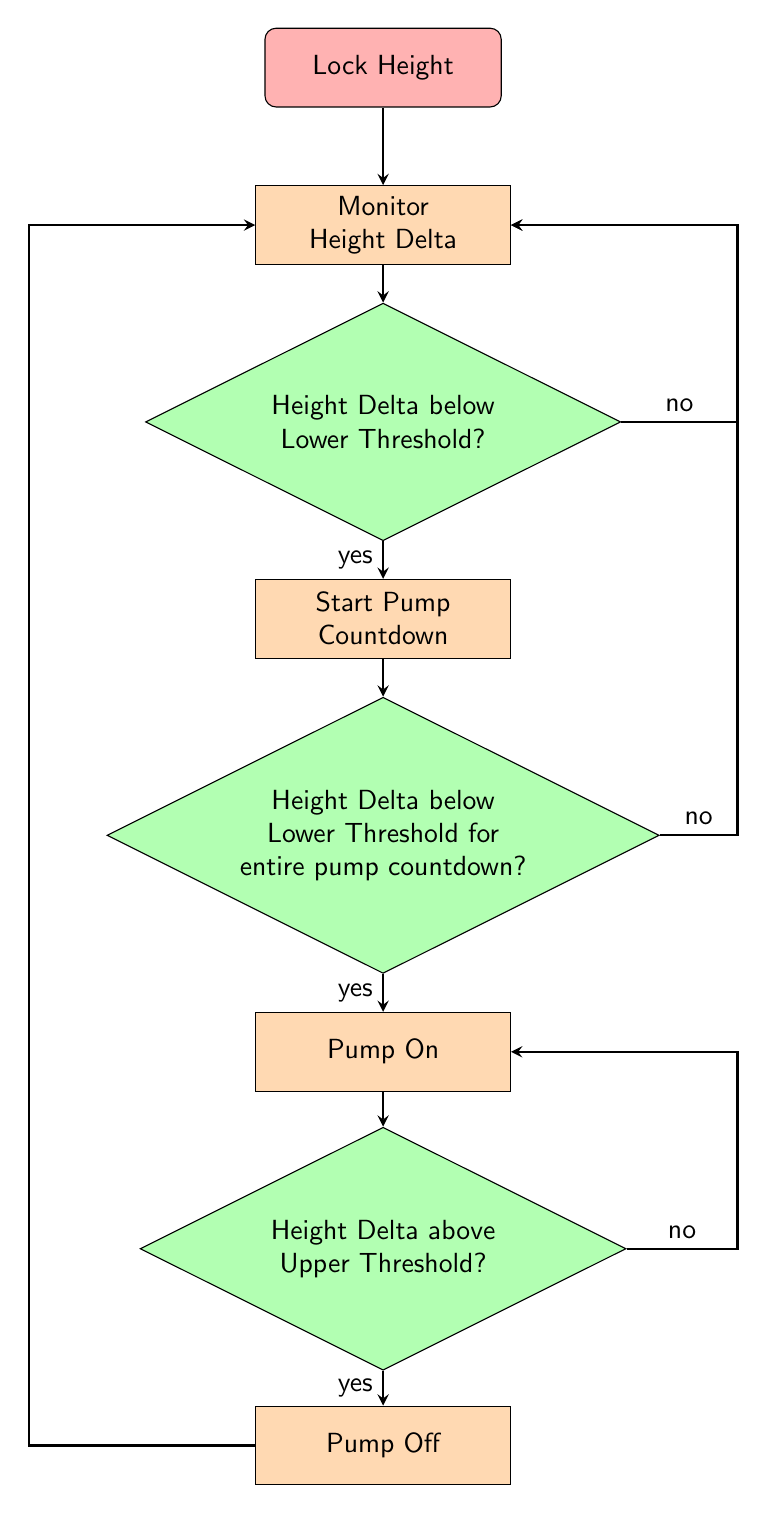
\begin{tikzpicture}[node distance=2cm]

\node (start) [startstop] {Lock Height};
\node (pro1) [process, below of=start] {Monitor Height Delta};
\node (dec1) [decision, below of=pro1, yshift=-0.5cm, aspect=2] {Height Delta below Lower Threshold?};
\node (pro2a) [process, below of=dec1, yshift=-0.5cm] {Start Pump Countdown};
\node (dec2) [decision, below of=pro2a, yshift=-0.75cm, aspect=2] {Height Delta below Lower Threshold for entire pump countdown?};
\node (pro3) [process, below of=dec2, yshift=-0.75cm] {Pump On};
\node (dec3) [decision, below of=pro3, yshift=-0.5cm, aspect=2] {Height Delta above Upper Threshold?};
\node (pro4) [process, below of=dec3, yshift=-0.5cm] {Pump Off};



\draw [arrow] (start) -- (pro1);
\draw [arrow] (pro1) -- (dec1);
\draw [arrow] (dec1) -- node[anchor=east] {yes} (pro2a);
\draw [arrow] (dec1) -- node[anchor=south] {no}  ++(4.5cm, 0cm) |- (pro1);
\draw [arrow] (dec2) -- node[anchor=south] {no}  ++(4.5cm, 0cm) |- (pro1);
\draw [arrow] (pro2a) -- (dec2);
\draw [arrow] (dec2) -- node[anchor=east] {yes} (pro3);
\draw [arrow] (pro3) -- (dec3);
\draw [arrow] (dec3) -- node[anchor=east] {yes} (pro4);
\draw [arrow] (dec3) -- node[anchor=south] {no} ++(4.5cm, 0cm) |- (pro3);
\draw [arrow] (pro4) -- ++(-4.5cm, 0cm) |- (pro1);

\end{tikzpicture}
\caption{Flowchart of the control logic for the pumping part of the LSHC.}\label{fig:flowchart}
\end{figure}

To briefly summarise what is shown in \autoref{fig:flowchart}, when the height of the liquid surface is at the desired position, the user will `lock' the height. Then the program will continually monitor the difference between the actual height and the locked height (this difference is the `height delta'). If the height delta falls below a given threshold (set by the user), then a countdown (set by the user) is started. This counts the number of `slow' frames that the height delta is below the threshold. If the height delta remains below the given threshold for the entire countdown, then the pump starts pumping at a speed set by the user. If at any point, one of the `fast' frames has a height delta which exceeds the upper threshold (set by the user), then the pump turns off. 

The effect of this is to ensure that the pump can only start on true evaporative loss and not a random fluctuation. However, the pump will turn off on a hair trigger - that is, any fluctuation where the height exceeds a given threshold will result in the pump turning off. This avoids the situation of `over-pumping', where the syringe overfills the sample holder and (less seriously) the user has to wait for the slow evaporative loss to bring the height back to the usable level; or (more seriously) the pump makes the sample holder overflow, potentially wasting lots of expensive sample. 

\subsection{LabVIEW Program}
The front panel from the LabVIEW program for controlling the LSHC is shown in \autoref{fig:frontpanel}. We will explain every item on the panel in turn. 

\begin{figure}
\centering
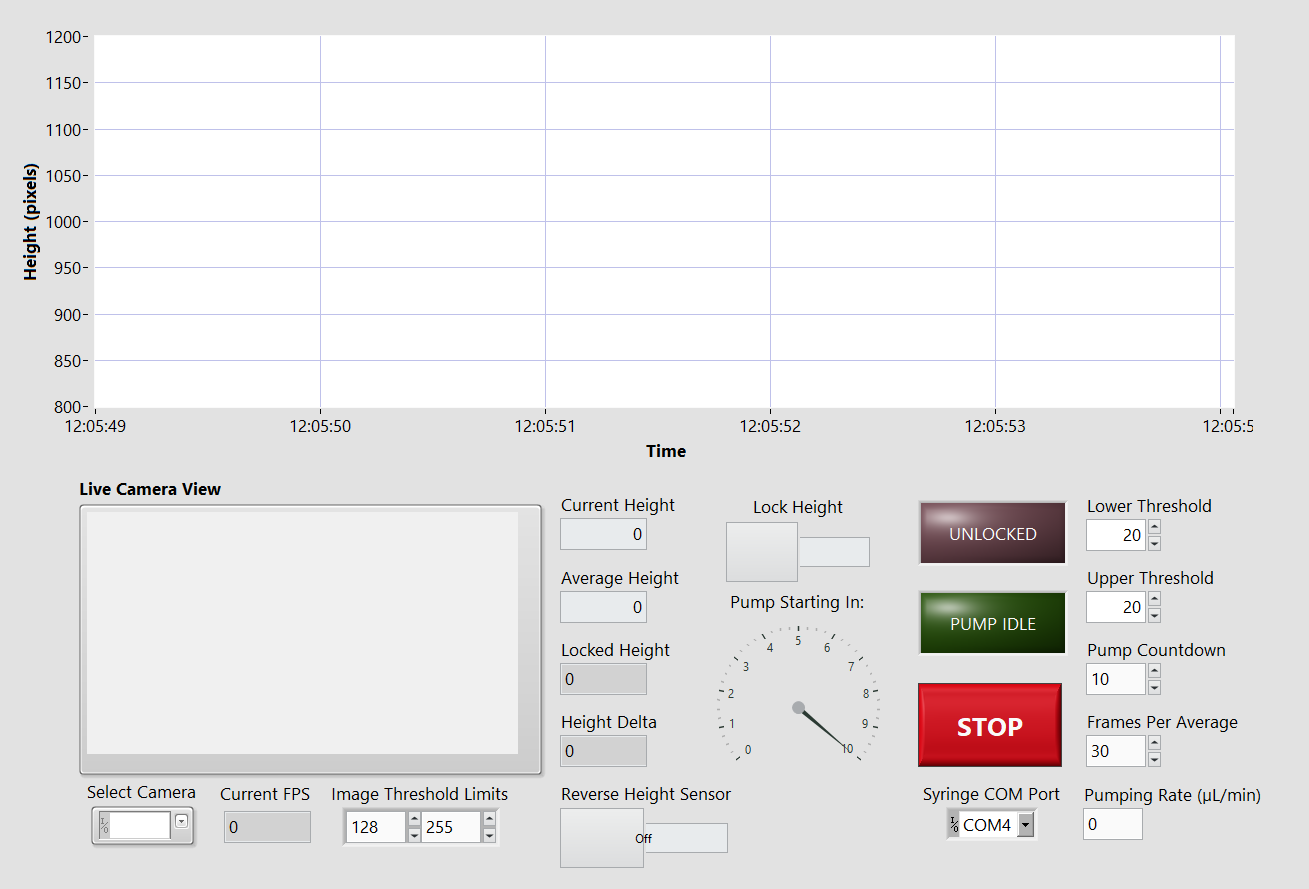
\includegraphics[width=\textwidth]{frontpanel_manual}
\caption{Front panel of the LabVIEW program for controlling the LSHC.}\label{fig:frontpanel}
\end{figure}
\begin{itemize}

\item \textbf{Top Graph:} a graph of height (in pixels) against time. When the program is running, this will display in real time the instantaneous height of the liquid surface (a grey line), and the average height (a red line). 
\item \textbf{Live Camera View:} a real time view of the webcam CCD. Useful to check if the beam hitting the sensor is round and uniform, or if the beam is close to missing the sensor. A crosshair on the live view shows the current center position.
\item \textbf{Select Camera:} selection box where the camera attached to the computer that is used for the LSHC can be selected.
\item \textbf{Current FPS:} the current repetition rate of the camera (in frames per second). 
\item \textbf{Image Threshold Limits:} applies thresholding to the image, boxes are lower (left) and upper (right). [0, 255] corresponds to no thresholding. Thresholding is useful if there is low intensity scattered light that causes the centre of the image to be unreliable.
\item \textbf{Reverse Height Sensor:} by default, the height sensor uses the long axis of the CCD as the `height' axis, but depending on the orientation of the camera, an increase in pixel position could correspond to a drop or fall in the height. This toggle switch allows the sensor to be `reversed' in software, so that an decrease in pixel position corresponds to an increase in sample height.
\item \textbf{Current Height:} the current height of the surface in pixels, read out at at the current FPS (normally \SI{30}{\hertz}).
\item \textbf{Average Height:} the average height of the surface in pixels, read out at the current FPS divded by Frames Per Average. Default is to \SI{1}{\hertz} with a \SI{30}{\hertz} camera.
\item \textbf{Locked Height:} the height of the surface at the point that the Lock Height toggle was pressed, in pixels.
\item \textbf{Height Delta:} the difference between the Current Height and the Locked Height, in pixels.
\item \textbf{Lock Height:} switching this toggle will store the Current Height as the Locked Height, and start the logic described in \autoref{fig:flowchart} to maintain the height using the syringe pump.
\item \textbf{Pump Starting In:} a countdown showing when the syringe pump will start. The countdown time is set using the Pump Countdown box. Shorter countdowns will cause faster compensation, but are more likely to start on a fluctuation than true evaporative loss.
\item \textbf{Unlocked LED:} an LED showing the current state of the LSHC. Switches from dull red when unlocked, to bright red when locked.
\item \textbf{Pump LED:} an LED showing the current state of the syringe pump. Switches from dull green when idle to bright green when pumping. 
\item \textbf{Stop Button:} stops the height sensor and syringe pump. 
\item \textbf{Syringe COM Port:} the COM port that the syringe pump is connected to. 
\item \textbf{Lower Threshold:} how far below the Locked Height the Height Delta has to be before the pump countdown starts, in pixels. 
\item \textbf{Upper Threshold:} how far above the Locked Height the Height Delta has to be before the pump will turn off, in pixels. 
\item \textbf{Pump Countdown:} the length of time the Height Delta needs to be below the Lower Threshold before the pump will engage, in number of average frames (in seconds using the default settings).
\item \textbf{Frames Per Average:} how many of the ´fast' frames to average into a `slow' frame. 
\item \textbf{Pumping Rate:}\footnote{This number tells the syringe pump how fast to drive, but the volume dispensed depends on the size of the syringe used. Here we assume a \SI{10}{\milli\litre} syringe, but in our experience this number should not be considered as entirely quantitative - trial and error in the \href{http://www.syringepump.com/software.php}{\underline{WinPumpTerm software}} is advised.} the speed at which the syringe pump pumps, in \si{\micro\litre\per\minute}.
\end{itemize} 

\section{Example Usage}
Finally we demonstrate how the LSHC software is used in practice with two examples. 
\subsection{Calibration}
The LSHC system and LabVIEW program works in height units of camera pixels, rather than in an absolute unit of length. The exact height change $\Delta h$ that a given change in position on the CCD $\Delta r$ corresponds to depends on the angle of incidence (AOI) of the incoming beam and is given by \autoref{eq:angle}. For a given experimental geometry, the change in CCD position $\Delta r$ that a given change in height $\Delta h$ corresponds to can be calculated by calibrating the LSHC. This is practically achieved by mounting a liquid sample on a micrometer stage, and then recording the position of the reflected beam on the CCD ($\Delta r$) as a function of the (known) change in height, $\Delta h$. Several data points can be collected and plotted, and then a linear fit to the points can be used for the calibration. An example of this is shown in \autoref{fig:calibration}.

\begin{figure}
\centering
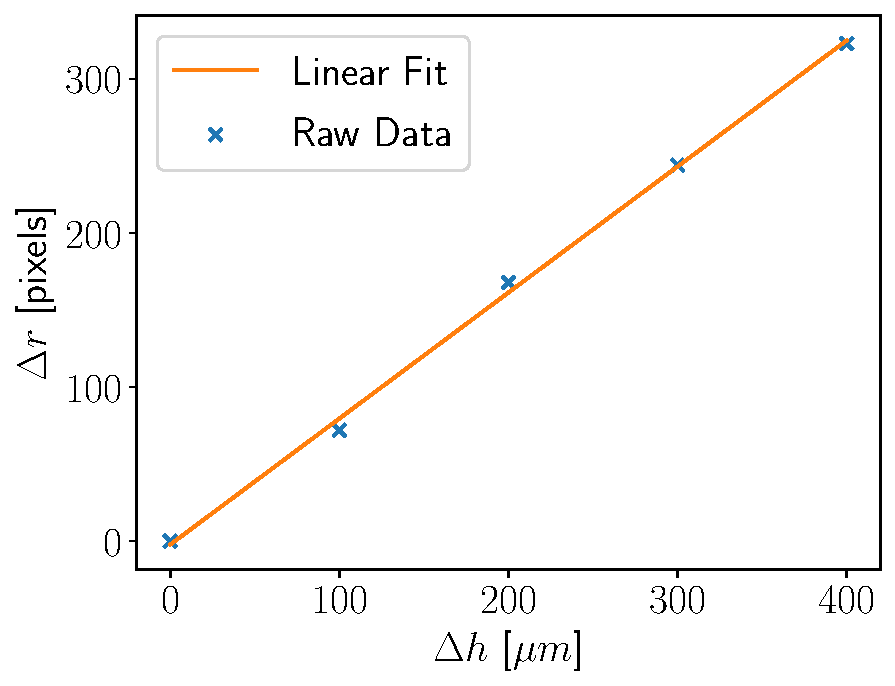
\includegraphics[width=0.8\textwidth]{calibration}
\caption{Plot of $\Delta h$ against $\Delta r$ for calibration purposes. Blue points show raw data, the orange line is a linear fit.}\label{fig:calibration}
\end{figure}

The gradient of the linear fit to the points in \autoref{fig:calibration} gives the calibration, and shows that moving the height by \SI{1}{\micro\metre} corresponds to the position of the beam on the CCD moving by 0.8 pixels, or conversely shows that a movement of 1 pixel on the CCD corresponds to \SI{1.25}{\micro\metre} of height movement. The centroiding process means that sub-pixel resolution of the camera height is possible, and a movement of the average centre by 0.8 pixels is certainly noticeable. From this calibration, one can conclude that the LSHC can notice and correct for changes in the height of less than \SI{1}{\micro\metre}. 

It is important to note that if a quantitative measure of the surface height is desired, then this calibration should be repeated every time the experimental setup is moved or rebuilt. However, we also note that it is entirely possible to use the LSHC without calibration, as the pixel pitch of the CCD provides a lower limit to the sensitivity. If the pixel pitch is \SI{2}{\micro\metre}, then the LSHC is sensitive to changes at least as small as this.

\subsection{Experimental Usage}
Here we present a simple walkthrough of using the LSHC software in practice. Initially, it is important to make sure that the COM port for the syringe, and camera name are both correct in the relevant i/o boxes. You can find out which ports are used in device manager, or NI MAX. Running the LabVIEW software will start the sensor and monitor the instantaneous and average height. This will be displayed on both the on-screen graph and the live camera view, as shown in \autoref{fig:panel_unlocked}. It may take some time to actually get the laser beam onto the sensor when initially setting up the device, and viewing the webcam output in NI MAX (or the standard system webcam viewer) can be easier than using the live feed from the LSHC software for this purpose. When the beam is found and roughly centered on the CCD sensor, adjustment of the two image threshold parameters can be used if needed to exclude any problematic ambient light.
\begin{figure}[h]
\centering
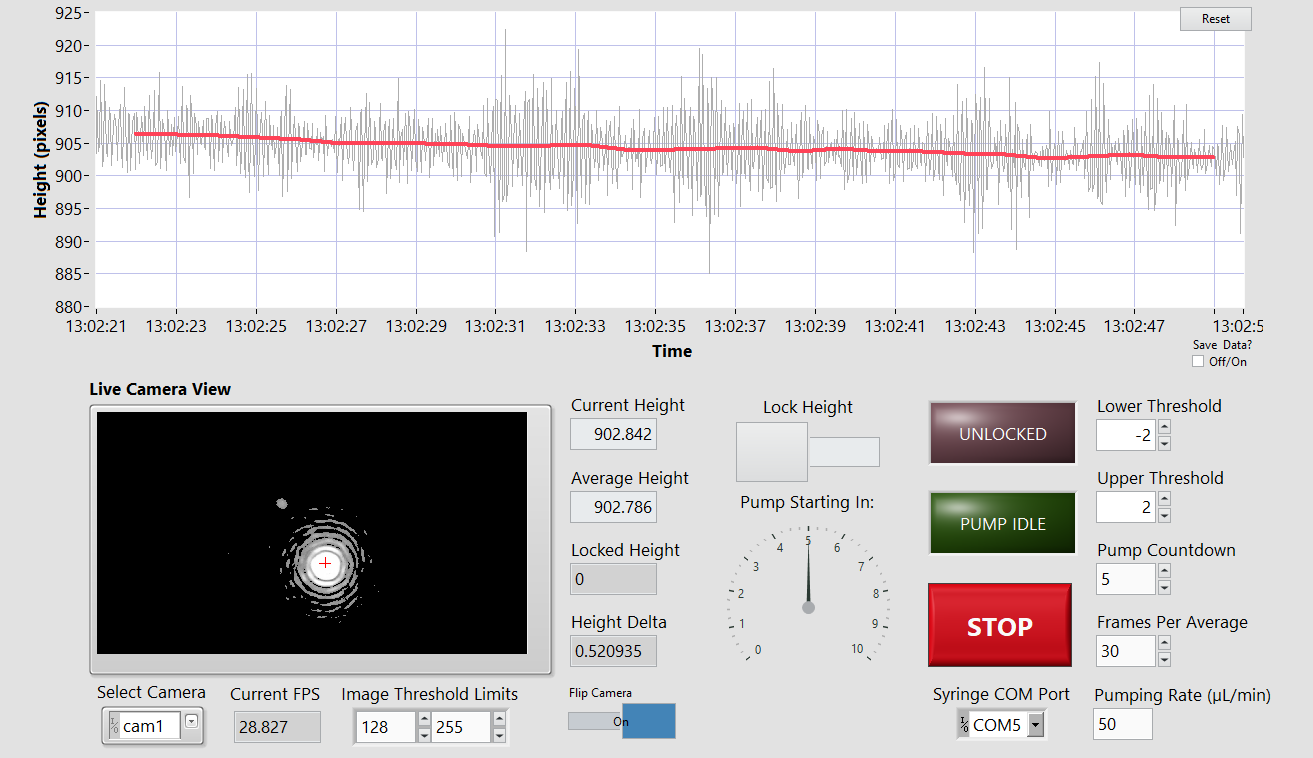
\includegraphics[width=0.8\textwidth]{panel_unlocked}
\caption{Front panel when height unlocked.}\label{fig:panel_unlocked}
\end{figure}
When the position of the beam is found, it is good practice to wait for a few minutes to check that the height of the surface drops over time due to evaporation. Depending on the orientation of the sensor, the software may read the drop in surface height as an increase in camera height, and it may be necessary to toggle the `Flip Height' switch to get this back to the expected behaviour. At this point you should also ensure that the upper and lower threshold, pump countdown, and pumping rate are all set to their desired values.  When this is done, the height can be locked by toggling the `Lock Height' switch. This changes the `Unlocked' LED to `Locked', and will initiate the syringe pump control logic to maintain the height at the position set when the `Lock Height' switch was toggled. The front panel just after the height has been locked is shown in \autoref{fig:panel_locked}. 
\begin{figure}[h]
\centering
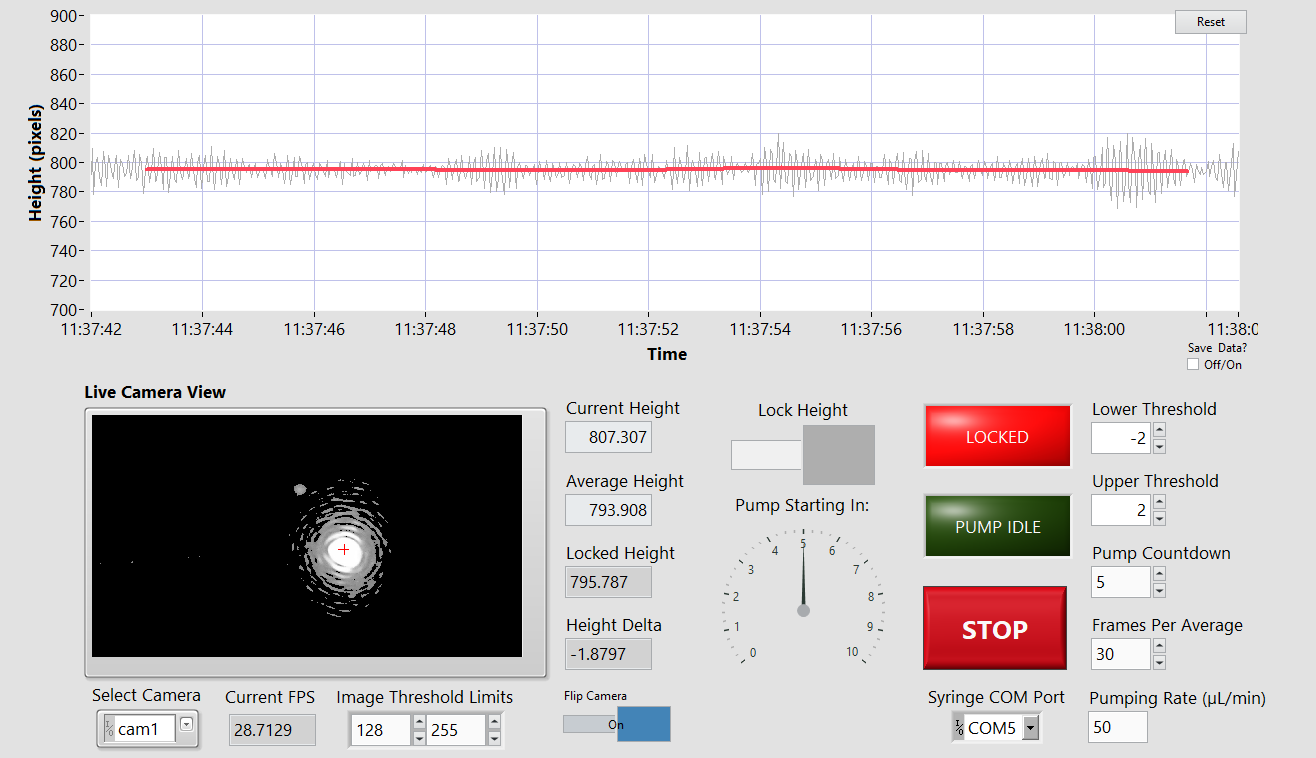
\includegraphics[width=0.8\textwidth]{panel_locked_nopump}
\caption{Front panel when height locked.}\label{fig:panel_locked}
\end{figure}
After a period of time, the height will drop due to evaporation, and once it has dropped by further than the lower threshold, the pump countdown will start. If the height delta remains below the lower threshold for the entire countdown, the syringe pump will activate. At this point, the green `Pump Idle' LED will illuminate and change to `Pumping'. This is shown in \autoref{fig:panel_pump}. The pump will remain active until the height delta is above the upper threshold, at which point the pump will deactivate (on the next average frame after the height delta is above the threshold). This cycle will continue indefinitely until the `Lock Height' switch is toggled again, or until the `STOP' button is pressed. Pressing `STOP' will both deactivate the pump and stop the software recording (and present an option to save the average and instantaneous height traces to a text file). If you simply need to adjust the height, or lock it at a new height, toggling the `Lock Height' switch is the best course of action. 
\begin{figure}[h]
\centering
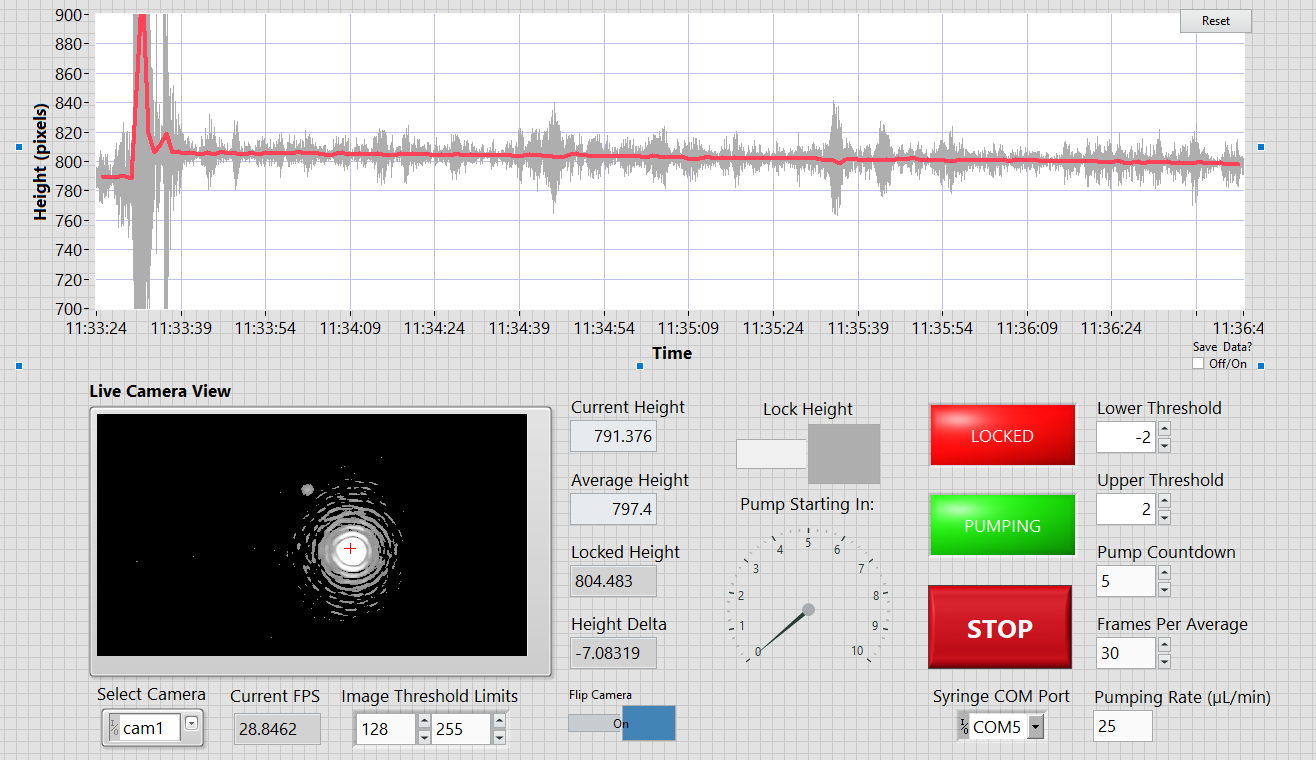
\includegraphics[width=0.8\textwidth]{panel_locked_pumping}
\caption{Front panel when height locked, and pump active.}\label{fig:panel_pump}
\end{figure}
When the experiment is complete, the LabVIEW can be stopped, and shut down safely. 

\end{document}